\section{Judul Penelitian}
Sistem Prediksi Lama Studi Mahasiswa Menggunakan Metode Jaringan Syaraf Tiruan.

\section{Bidang Ilmu}
Bidang ilmu yang berkaitan dengan penelitian ini adalah Kecerdasan Buatan (\textit{Artificial Intelligence}).

\section{Latar Belakang}
Lama studi mahasiswa merupakan salah satu indikator penting yang mencerminkan kualitas dan efektivitas pendidikan di perguruan tinggi. Durasi penyelesaian studi tidak hanya berdampak pada mahasiswa secara individual, tetapi juga memiliki implikasi signifikan bagi institusi pendidikan tinggi secara keseluruhan. Semakin cepat dan tepat waktu mahasiswa menyelesaikan studinya, semakin baik pula kinerja institusi dalam menjalankan fungsi pendidikannya. Hal ini sejalan dengan temuan \cite{so2020developing} yang menyatakan bahwa ketepatan waktu kelulusan mahasiswa merupakan perhatian utama bagi penyelenggara pendidikan tinggi, terutama bagian urusan kemahasiswaan, dalam merancang kegiatan pengembangan yang bermakna dan diterima dengan baik oleh mahasiswa. Lebih lanjut, \cite{chen2019analysis} menggarisbawahi pentingnya analisis durasi studi mahasiswa bagi institusi pendidikan tinggi untuk mengidentifikasi faktor-faktor yang mempengaruhi lama studi dan mengembangkan strategi untuk meningkatkan tingkat kelulusan tepat waktu. Kedua penelitian ini menekankan bahwa pemahaman tentang faktor-faktor yang mempengaruhi lama studi mahasiswa dapat membantu institusi pendidikan tinggi dalam mengembangkan strategi yang efektif untuk meningkatkan tingkat kelulusan tepat waktu dan mengurangi angka putus kuliah.

Pentingnya ketepatan waktu kelulusan telah dipahami dengan baik, realitas di lapangan menunjukkan bahwa masih banyak mahasiswa yang tidak dapat menyelesaikan studi mereka sesuai dengan waktu yang ditentukan. Fenomena ini menjadi permasalahan serius yang perlu ditangani oleh institusi pendidikan tinggi. Keterlambatan kelulusan tidak hanya berdampak pada efisiensi sistem pendidikan, tetapi juga memiliki konsekuensi ekonomi dan sosial yang signifikan bagi mahasiswa dan masyarakat secara luas. Menurut \cite{putri2018analysis}, tingkat kelulusan tepat waktu di beberapa perguruan tinggi masih berada di bawah 50\%, yang menunjukkan adanya gap yang besar antara harapan dan kenyataan. Lebih lanjut, \cite{wang2018design} mengidentifikasi bahwa keterlambatan kelulusan sering kali disebabkan oleh berbagai faktor kompleks, termasuk permasalahan akademik, finansial, dan psikososial yang dihadapi mahasiswa selama masa studi mereka. Oleh karena itu, identifikasi dini terhadap mahasiswa yang berisiko mengalami keterlambatan kelulusan menjadi sangat penting untuk memungkinkan intervensi yang tepat waktu dan efektif.

Masalah keterlambatan kelulusan mahasiswa dapat diatasi dengan mengembangkan dan menerapkan sistem bimbingan akademik sebagai solusi konvensional. Sistem bimbingan akademik ini bertujuan untuk membantu mahasiswa mengatasi tantangan akademik dan pribadi, serta mengarahkan mereka menuju jalur pendidikan tinggi yang telah mereka pilih. Seperti yang dikemukakan oleh \cite{elcullada2018academic}, bimbingan akademik dianggap sebagai bagian penting dari keberhasilan akademik mahasiswa. Namun, sistem bimbingan konvensional seringkali menghadapi berbagai kendala, seperti beban kerja dosen pembimbing yang tinggi, waktu pertemuan yang terbatas, dan kurangnya pemahaman menyeluruh tentang latar belakang mahasiswa. Hal ini dapat mengakibatkan kualitas bimbingan yang kurang optimal dan mahasiswa membuat pilihan akademik yang kurang tepat. 

Berbagai pendekatan telah diusulkan dan diterapkan untuk memprediksi lama studi mahasiswa dalam beberapa tahun terakhir. \cite{alyahyan2020decision} mengembangkan model prediksi menggunakan algoritma pohon keputusan, khususnya J48, Random Tree, dan REPTree. Mereka memanfaatkan data akademik mahasiswa seperti nilai mata kuliah dan IPK tahun pertama untuk memprediksi prestasi akademik mahasiswa di akhir masa studi. Model terbaik yang dihasilkan mampu mencapai akurasi hingga 69,3\%. Sementara itu, \cite{danbatta2020predicting} menerapkan beberapa teknik regresi seperti regresi linear, eksponensial, logaritmik, polinomial dan power untuk memprediksi IPK akhir mahasiswa berdasarkan IPK tahun pertama. Mereka menemukan bahwa regresi linear memberikan hasil terbaik dengan tingkat akurasi yang cukup tinggi. Pendekatan berbeda diambil oleh \cite{olalekan2020performance} yang membandingkan kinerja Naive Bayes dan Jaringan Syaraf Tiruan (JST) dalam memprediksi kelulusan mahasiswa. Hasil penelitian mereka menunjukkan bahwa JST mampu menghasilkan akurasi yang lebih tinggi, mencapai 79,31\% untuk satu lapisan tersembunyi dan meningkat hingga 99,97\% untuk empat lapisan tersembunyi.

Berdasarkan tinjauan dari beberapa penelitian yang telah dilakukan, berbagai pendekatan telah diusulkan untuk memprediksi lama studi mahasiswa menggunakan metode Jaringan Syaraf Tiruan (JST), khususnya algoritma backpropagation. \cite{hossen2021web} mengembangkan model prediksi berbasis web dengan arsitektur empat tingkat menggunakan JST. Mereka menerapkan seleksi fitur untuk mengurangi jumlah variabel input dari 15 menjadi 4, yang menghasilkan peningkatan akurasi dan efisiensi komputasi. Model terbaik mereka mencapai akurasi 92\% menggunakan 4 fitur teratas. Sementara itu, \cite{sunardi2022pengaruh} melakukan analisis mendalam terhadap pengaruh jumlah hidden layer dan learning rate pada kecepatan pelatihan JST backpropagation. Mereka menemukan bahwa arsitektur dengan 12 neuron di hidden layer memberikan waktu pelatihan tercepat yaitu 3 menit 44 detik. Learning rate optimal yang mereka temukan adalah 0,5 dengan 100.000 iterasi. Pendekatan berbeda diambil oleh \cite{sari2021analisis} yang fokus pada prediksi mahasiswa dropout. Mereka membandingkan beberapa arsitektur JST dan menemukan bahwa model 12-5-2 (12 input, 5 hidden, 2 output) memberikan akurasi terbaik sebesar 98,2\% dengan learning rate 0,4 dan momentum 0,95. Ketiga studi tersebut menunjukkan bahwa optimalisasi parameter JST seperti arsitektur jaringan, jumlah neuron hidden layer, learning rate, dan momentum sangat penting untuk meningkatkan akurasi dan efisiensi model prediksi lama studi mahasiswa.

Oleh karena itu, penelitian ini mengusulkan pengembangan sistem prediksi lama studi mahasiswa menggunakan metode Jaringan Syaraf Tiruan (JST) dengan algoritma backpropagation. Sistem yang diusulkan akan mengintegrasikan data pembelajaran dari \textit{e-learning}, khususnya data pembelajaran mahasiswa TI \& SI tahun 2022 yang relevan. Penelitian ini akan fokus pada optimalisasi arsitektur jaringan, penentuan jumlah neuron pada hidden layer yang optimal, serta pencarian nilai learning rate dan momentum yang tepat untuk meningkatkan akurasi prediksi. Selain itu, akan dilakukan perbandingan kinerja model JST dengan metode machine learning lainnya untuk memvalidasi efektivitas pendekatan yang diusulkan. Diharapkan hasil penelitian ini dapat memberikan alat prediksi yang akurat dan efisien bagi institusi pendidikan tinggi untuk mengidentifikasi mahasiswa yang berisiko mengalami keterlambatan studi, sehingga intervensi dini dapat dilakukan untuk meningkatkan tingkat kelulusan tepat waktu.

\section{Rumusan Masalah}
Berdasarkan latar belakang yang telah diuraikan, rumusan masalah dalam penelitian ini adalah sebagai berikut:
    \begin{enumerate}
        \item Bagaimana mengembangkan sistem prediksi lama studi mahasiswa menggunakan metode Jaringan Syaraf Tiruan (JST) dengan algoritma backpropagation berdasarkan data pembelajaran e-learning mahasiswa TI \& SI tahun 2022?
        \item Bagaimana mengoptimalkan arsitektur jaringan, jumlah neuron pada hidden layer, nilai learning rate, dan momentum untuk meningkatkan akurasi prediksi lama studi mahasiswa menggunakan data e-learning?
        \item Bagaimana kinerja model JST yang dikembangkan dibandingkan dengan metode machine learning lainnya dalam memprediksi lama studi mahasiswa berdasarkan data e-learning?
    \end{enumerate}

\section{Batasan Masalah}
Untuk memfokuskan penelitian ini, beberapa batasan masalah ditetapkan sebagai berikut:
    \begin{enumerate}
        \item Penelitian ini fokus pada penggunaan metode Jaringan Syaraf Tiruan (JST) dengan algoritma backpropagation untuk memprediksi lama studi mahasiswa.
        \item Data yang digunakan dalam penelitian ini terbatas pada data pembelajaran e-learning mahasiswa TI \& SI tahun 2022.
        \item Optimalisasi model JST akan dilakukan pada parameter arsitektur jaringan, jumlah neuron hidden layer, learning rate, dan momentum menggunakan data e-learning.
        \item Perbandingan kinerja akan dilakukan antara model JST yang dikembangkan dengan beberapa metode machine learning lainnya yang umum digunakan untuk prediksi menggunakan data e-learning.
    \end{enumerate}

\section{Tujuan Penelitian}
Tujuan dari penelitian ini adalah:
    \begin{enumerate}
        \item Mengembangkan sistem prediksi lama studi mahasiswa menggunakan metode Jaringan Syaraf Tiruan (JST) dengan algoritma backpropagation berdasarkan data pembelajaran e-learning mahasiswa TI \& SI tahun 2022.
        \item Mengoptimalkan arsitektur jaringan, jumlah neuron pada hidden layer, nilai learning rate, dan momentum untuk meningkatkan akurasi prediksi lama studi mahasiswa menggunakan data e-learning.
        \item Membandingkan kinerja model JST yang dikembangkan dengan metode machine learning lainnya dalam memprediksi lama studi mahasiswa berdasarkan data e-learning.
    \end{enumerate}

\section{Manfaat Penelitian}
Penelitian ini diharapkan dapat memberikan manfaat sebagai berikut:

    \begin{enumerate}
        \item Memberikan kontribusi dalam pengembangan sistem prediksi lama studi mahasiswa berbasis data e-learning yang dapat diimplementasikan di institusi pendidikan tinggi.
        \item Meningkatkan pemahaman tentang faktor-faktor dalam pembelajaran e-learning yang mempengaruhi lama studi mahasiswa dan bagaimana memprediksinya menggunakan metode Jaringan Syaraf Tiruan.
        \item Menyediakan alat bantu bagi institusi pendidikan tinggi untuk mengidentifikasi mahasiswa yang berisiko mengalami keterlambatan studi berdasarkan performa e-learning mereka, sehingga dapat dilakukan intervensi dini.
        \item Berkontribusi pada peningkatan efisiensi dan efektivitas sistem pendidikan tinggi melalui prediksi lama studi yang lebih akurat berdasarkan data e-learning.
        \item Memperkaya literatur ilmiah tentang aplikasi metode Jaringan Syaraf Tiruan dalam analisis data e-learning, khususnya untuk prediksi lama studi mahasiswa.
        \item Memberikan landasan untuk penelitian lebih lanjut dalam pengembangan sistem prediksi dan analisis data e-learning menggunakan metode machine learning.
    \end{enumerate}

\section{Tinjauan Pustaka}
\begin{enumerate}
    \item \textbf{Lama Studi Mahasiswa dan Dampaknya}
    
    Lama studi mahasiswa merupakan indikator penting yang mencerminkan kualitas dan efektivitas pendidikan tinggi, serta memiliki dampak signifikan baik bagi mahasiswa maupun institusi. Ketepatan waktu kelulusan tidak hanya menjadi perhatian utama bagi penyelenggara pendidikan tinggi dalam merancang kegiatan pengembangan yang bermakna, tetapi juga menjadi salah satu kriteria penilaian akreditasi oleh Badan Akreditasi Nasional Perguruan Tinggi (BAN-PT) \cite{wirawan2019application}. Keterlambatan kelulusan dapat mengakibatkan berbagai konsekuensi negatif, seperti penurunan efisiensi sistem pendidikan, penumpukan mahasiswa, serta implikasi ekonomi dan sosial bagi mahasiswa dan masyarakat luas. Hal ini dipertegas oleh temuan bahwa tingkat kelulusan tepat waktu di beberapa perguruan tinggi masih berada di bawah 50\%, menunjukkan adanya kesenjangan antara harapan dan realitas \cite{dengen2018student}. Oleh karena itu, pemahaman mendalam tentang faktor-faktor yang mempengaruhi lama studi mahasiswa dan pengembangan strategi untuk meningkatkan tingkat kelulusan tepat waktu menjadi sangat penting bagi institusi pendidikan tinggi dalam upaya meningkatkan kualitas pendidikan dan mempertahankan akreditasi yang baik.

    \item \textbf{Machine Learning}
    
    Machine learning, sebagai cabang kecerdasan buatan, memungkinkan sistem komputer untuk belajar dan meningkatkan kinerja dari pengalaman tanpa pemrograman eksplisit. Ray \cite{ray2019quick} menjelaskan bahwa pendekatan machine learning umumnya terbagi menjadi beberapa kategori utama, termasuk pembelajaran terbimbing, tak terbimbing, semi-terbimbing, dan pembelajaran penguatan. Setiap pendekatan ini memiliki karakteristik dan aplikasi yang berbeda, memungkinkan penggunaan machine learning dalam berbagai bidang. Gupta dan Roman-Gonzalez \cite{gupta2020survey} memperluas pemahaman ini dengan menunjukkan aplikasi luas machine learning, mulai dari pengenalan pola hingga analisis prediktif, yang mencerminkan fleksibilitas dan kekuatan teknologi ini dalam menangani berbagai jenis data dan permasalahan.

    \item \textbf{Jaringan Syaraf Tiruan}
    
    Jaringan Syaraf Tiruan (JST) adalah sistem komputasi yang terinspirasi dari prinsip kerja jaringan syaraf biologis otak manusia. JST terdiri dari sejumlah besar unit pemrosesan sederhana yang saling terhubung, disebut neuron artifisial, yang bekerja secara paralel untuk memproses informasi dan menghasilkan output berdasarkan input yang diterima. Setiap koneksi antar neuron memiliki bobot yang dapat dimodifikasi melalui proses pembelajaran, memungkinkan JST untuk beradaptasi dan mempelajari pola dari data yang diberikan. Arsitektur dasar JST terdiri dari lapisan input, satu atau lebih lapisan tersembunyi, dan lapisan output, dengan setiap neuron memiliki fungsi aktivasi yang menentukan outputnya berdasarkan input yang diterima. Salah satu keunggulan utama JST adalah kemampuannya untuk melakukan generalisasi dan menangani masalah non-linear, membuatnya cocok untuk berbagai aplikasi seperti pengenalan pola, klasifikasi, prediksi, dan pengambilan keputusan. Implementasi digital JST, terutama menggunakan FPGA, menawarkan keuntungan dalam hal kecepatan komputasi dan kemampuan rekonfigurasi, meskipun memerlukan pertimbangan khusus dalam hal representasi bobot, implementasi fungsi aktivasi, dan algoritma pembelajaran seperti backpropagation \cite{amrutha2018performance}.

    \item \textbf{Sistem Prediksi}
    
    Sistem prediksi adalah suatu pendekatan komputasional yang dirancang untuk memperkirakan atau meramalkan hasil atau kejadian di masa depan berdasarkan analisis data historis dan pola yang ada. Sistem ini menggunakan berbagai teknik dan algoritma, termasuk metode statistik, machine learning, dan kecerdasan buatan, untuk mengidentifikasi tren, pola, dan hubungan dalam data yang dapat digunakan untuk membuat perkiraan yang akurat \cite{dengen2018student}. Penerapan sistem prediksi mencakup berbagai bidang, mulai dari peramalan cuaca dan analisis pasar keuangan hingga prediksi perilaku konsumen dan hasil akademik mahasiswa. Dalam konteks pendidikan tinggi, sistem prediksi dapat digunakan untuk mengidentifikasi mahasiswa yang berisiko mengalami keterlambatan kelulusan atau putus kuliah, memungkinkan institusi untuk mengambil tindakan preventif dan memberikan dukungan yang diperlukan \cite{wirawan2019application}. Keakuratan dan kehandalan sistem prediksi sangat bergantung pada kualitas data yang digunakan, pemilihan fitur yang relevan, dan kesesuaian algoritma yang diterapkan dengan karakteristik masalah yang dihadapi.
\end{enumerate}

\section{Metode Penelitian}

\begin{enumerate}
    \item \textbf{Jenis Penelitian}
    
    Penelitian ini mengadopsi pendekatan penelitian terapan, dengan fokus utama pada implementasi teknologi Jaringan Syaraf Tiruan dalam pengembangan sistem prediksi lama studi mahasiswa. Melalui pendekatan ini, penelitian bertujuan untuk mengaplikasikan dan mengevaluasi efektivitas metode Jaringan Syaraf Tiruan dalam konteks spesifik sistem perdiksi lama studi mahasiswa.

    \item \textbf{Waktu dan Tempat Penelitian}
    
    Penelitian ini dilaksanakan dalam rentang waktu empat bulan, dimulai dari Agustus 2024 hingga November 2024. Pengumpulan data dilakukan melalui akuisisi dataset dari Program Studi Sistem Informasi dan Informatika yang menyediakan basis data komprehensif mengenai data-data pembelajaran e-learning mahasiswa yang akan digunakan untuk membuat prediksi lama studi.

    \item \textbf{Sarana dan Pendukung}
    
    Untuk memastikan keberhasilan dan efisiensi penelitian ini, berbagai sarana pendukung telah diidentifikasi dan disiapkan. Perangkat keras dan perangkat lunak yang dipilih tidak hanya mendukung pelaksanaan penelitian, tetapi juga memungkinkan pengembangan dan pengujian sistem prediksi secara optimal. Berikut adalah rincian perangkat yang digunakan:

    \begin{enumerate}
        \item Perangkat Keras
        \begin{itemize}
            \item Memori RAM 8GB DDR3, yang menyediakan kapasitas yang memadai untuk pemrosesan data dan eksekusi model.
            \item Penyimpanan SSD 256GB, memungkinkan akses data yang cepat dan efisien, serta mempercepat proses komputasi.
        \end{itemize}

        \item Perangkat Lunak
        \begin{itemize}
            \item Python versi 3 atau lebih tinggi, dipilih sebagai bahasa pemrograman utama untuk pengembangan dan implementasi model machine learning.
            \item Flask, framework web Python yang ringan dan fleksibel, digunakan untuk mengekspos model sebagai API, memfasilitasi integrasi dengan komponen sistem lainnya.
            \item Node.js, platform JavaScript server-side yang kuat, berfungsi sebagai backend untuk mengelola logika aplikasi dan alur data.
            \item React.js, library JavaScript modern untuk pengembangan antarmuka pengguna, dipilih untuk menciptakan pengalaman pengguna yang responsif dan interaktif.
            \item Figma, alat desain kolaboratif berbasis web, digunakan untuk merancang dan memprototype antarmuka pengguna sistem.
            \item Draw.io (App Diagram), platform pembuatan diagram online, dimanfaatkan untuk merancang dan mendokumentasikan arsitektur sistem melalui diagram UML.
        \end{itemize}
    \end{enumerate}

    \item \textbf{Rancangan Penelitian}
    
    Rancangan penelitian ini disusun secara sistematis untuk memastikan pelaksanaan yang terstruktur dan efektif. Dengan mengadopsi metodologi \textit{Cross-Industry Standard Process for Data Mining} (CRISP-DM), penelitian ini dibagi menjadi beberapa tahapan kritis yang saling terkait. Setiap tahapan dirancang untuk membangun fondasi bagi tahapan berikutnya, memastikan kesinambungan dalam proses penelitian. Alur metode ini dapat dilihat pada Gambar \ref{fig:crisp-dm-overview}.

    \begin{figure}[htbp]
        \centering
        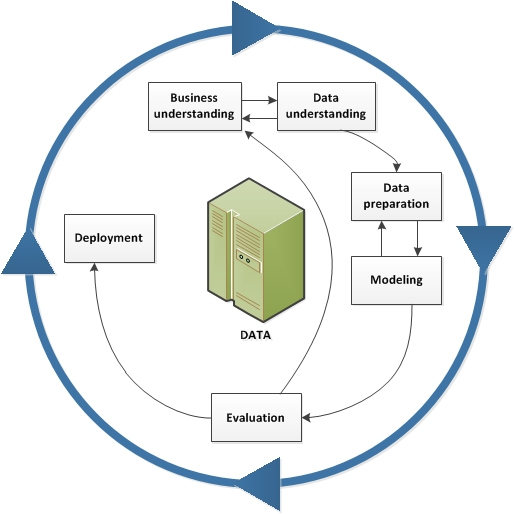
\includegraphics[width=0.5\textwidth]{images/crisp-dm-overview.jpg}
        \caption{Alur Metode CRISP-DM \cite{IBM2022}}
        \label{fig:crisp-dm-alur}
    \end{figure}

    Gambar \ref{fig:crisp-dm-overview} mengilustrasikan alur metode CRISP-DM yang diterapkan dalam pengembangan Sistem Prediksi Lama Studi Mahasiswa menggunakan Metode Jaringan Syaraf Tiruan. Berikut adalah penjelasan setiap tahap dalam konteks penelitian ini:

    \begin{enumerate}
        \item \textit{Business Understanding}
        
        Tahap ini berfokus pada pemahaman mendalam tentang kebutuhan dan tantangan dalam memprediksi lama studi mahasiswa di institusi pendidikan tinggi. Melalui wawancara dengan \textit{stakeholder} akademik seperti dosen pembimbing, tujuan spesifik dari sistem prediksi yang akan dikembangkan menggunakan Jaringan Syaraf Tiruan akan didefinisikan dengan jelas. Pemahaman ini akan menjadi landasan untuk merancang solusi prediksi yang akurat, tepat sasaran, dan bernilai tinggi bagi institusi dalam upaya meningkatkan tingkat kelulusan tepat waktu dan mengurangi angka putus kuliah.

        \item \textit{Data Understanding}
        
        Pada tahap ini, dilakukan eksplorasi mendalam terhadap dataset akademik mahasiswa yang tersedia. Aktivitas ini mencakup analisis statistik deskriptif, visualisasi data, dan identifikasi pola yang mungkin mempengaruhi lama studi mahasiswa. Dataset yang akan dieksplorasi meliputi data akademik seperti IPK per semester, nilai mata kuliah, dan data demografis mahasiswa. Pemahaman yang baik tentang karakteristik data, termasuk kualitas, kelengkapan, dan relevansinya terhadap prediksi lama studi, akan membantu dalam merancang strategi \textit{preprocessing} yang efektif dan pemilihan fitur yang tepat untuk model Jaringan Syaraf Tiruan. Analisis korelasi antar variabel juga akan dilakukan untuk mengidentifikasi faktor-faktor yang memiliki pengaruh signifikan terhadap lama studi mahasiswa.

        \item \textit{Data Preparation}
        
        Tahap persiapan data melibatkan serangkaian proses untuk mengolah data akademik mahasiswa menjadi format yang siap digunakan dalam pemodelan Jaringan Syaraf Tiruan. Kegiatan ini mencakup pembersihan data untuk mengatasi nilai yang hilang atau tidak konsisten pada \textit{record} akademik, normalisasi atau standarisasi fitur numerik seperti IPK dan nilai mata kuliah, \textit{encoding} variabel kategorikal seperti jurusan atau status mahasiswa, dan \textit{feature engineering} untuk menciptakan fitur baru yang lebih informatif, misalnya rata-rata nilai mata kuliah inti. Selain itu, dataset akan dibagi menjadi set pelatihan dan pengujian untuk memfasilitasi evaluasi model prediksi lama studi yang akurat.

        \item \textit{Modeling}
        
        Dalam tahap pemodelan, implementasi metode Jaringan Syaraf Tiruan dengan algoritma \textit{backpropagation} untuk memprediksi lama studi mahasiswa akan dilakukan. Proses ini melibatkan eksperimen dengan berbagai arsitektur jaringan, penentuan jumlah \textit{layer} dan neuron yang optimal, serta \textit{tuning hyperparameter} seperti \textit{learning rate} dan momentum. Validasi silang akan digunakan untuk mengoptimalkan performa model. Fokus utama adalah pada pengembangan model JST yang dapat menangkap kompleksitas hubungan antara berbagai faktor akademik dan non-akademik yang mempengaruhi lama studi mahasiswa.

        \item \textit{Evaluation}
        
        Evaluasi model JST akan dilakukan secara komprehensif menggunakan berbagai metrik kinerja seperti \textit{Mean Absolute Error} (MAE), \textit{Root Mean Square Error} (RMSE), dan koefisien determinasi (R²) untuk mengukur akurasi prediksi lama studi. Selain itu, analisis sensitivitas akan dilakukan untuk memahami pengaruh relatif dari berbagai input terhadap prediksi. Proses evaluasi ini juga akan mencakup perbandingan dengan metode \textit{machine learning} lainnya seperti regresi linear dan \textit{decision tree} untuk mengukur keunggulan pendekatan JST dalam konteks prediksi lama studi mahasiswa.

        \item \textit{Deployment}
        
        Setelah model JST final dipilih dan divalidasi, tahap \textit{deployment} akan fokus pada integrasi model ke dalam sistem informasi akademik yang ada di institusi. Ini melibatkan pengembangan antarmuka pengguna yang \textit{user-friendly} untuk staf akademik, implementasi \textit{backend} untuk menjalankan prediksi, dan penyiapan API untuk mengintegrasikan fungsionalitas prediksi dengan sistem yang ada.
    \end{enumerate}

    \item \textbf{Jadwal Penelitian}
    
    Jadwal dan waktu pelaksanaan penelitian ini dapat dilihat pada Tabel \ref{tab:jadwal-penelitian}. 

    \begin{table}[htbp]
        \centering
        \setlength{\tabcolsep}{4pt}
        \renewcommand{\arraystretch}{1.2}
        \caption{Jadwal Kegiatan Penelitian}
        \label{tab:jadwal-penelitian}
        \begin{tabular}{|c|p{4cm}|c|c|c|c|}
        \hline
        \multirow{2}{*}{\textbf{No}} & \multirow{2}{*}{\textbf{Kegiatan}} & \multicolumn{4}{c|}{\textbf{Bulan}} \\
        \cline{3-6}
         & & \textbf{Agustus} & \textbf{September} & \textbf{Oktober} & \textbf{November} \\
        \hline
        1. & Studi pustaka & \cellcolor{lightgray} & & & \\
        \hline
        2. & Penerimaan proposal & \cellcolor{lightgray} & \cellcolor{lightgray} & & \\
        \hline
        3. & Pengumpulan dan analisis data & \cellcolor{lightgray} & \cellcolor{lightgray} & & \\
        \hline
        4. & Pembuatan sistem & & \cellcolor{lightgray} & \cellcolor{lightgray} & \\
        \hline
        5. & Pengujian hasil & & & \cellcolor{lightgray} & \\
        \hline
        6. & Penyelesaian laporan dan aplikasi akhir & & & \cellcolor{lightgray} & \cellcolor{lightgray} \\
        \hline
        \end{tabular}
    \end{table}
\end{enumerate}

\begin{landscape}
\section{Penelitian Terkait}
\mbox{} % Membuat halaman pertama tetap kosong
\end{landscape}
